\subsection{Random Access Memory}

\subsubsection{RAM access time}
\paragraph{Methodology}
We measured the back-to-back-load RAM access latency, because it is well accepted by most software developers and system researchers.
We use the method described in the paper \emph{lmbench: Portable Tools for Performance Analysis} to measure the memory and cache latency.
We create arrays of different sizes, we create a list of pointers to walk the list and then we walk the list like this :
\begin{verbatim}
p = *p;
\end{verbatim}

Then we created the list with different strides and did the same measurement.
For each couple of stride/array sizes we do 1,000,000 iterates through the list.
The value of the pointer p is then printed to avoid that the compiler optimize the loop and remove the instruction.

\paragraph{Predictions}
According to the \emph{Intel® 64 and IA-32 Architectures Optimization Reference Manual}
\ref{intel-archi-opti-intel64} base case latencies are :
\begin{description}
\item[L1 cache] 4 cycles
\item[L2 cache] 12 cycles
\item[L3 cache] 28 cycles
\item[Main memory] 45 cycles
\end{description}
According to the RAM specification the latency is about 15ns.
It's about 45 cpu cycles as the CPU is running at 3.3Ghz. Because of the way our measurement is setup, there is no software cost involved in this case.


\paragraph{Results}
We are going to present the result table for stride 11 and the plotted graph for different strides from 1 to 15.

\begin{table}[h]
\begin{center}
\begin{tabular}{| r | l | l | l | r |}
\hline
Size of array 	& Hardware cost 	& Software cost 	& Prediction 	& Measured \\ \hline
512B 			&	4 cycles		&	0 cycle		&	4 cycles	&3.895 cycles	\\ \hline
1KB 			&	4 cycles		&	0 cycle		&	4 cycles	&3.886 cycles		\\ \hline
2KB 			&	4 cycles		&	0 cycle		&	4 cycles	&3.885 cycles		\\ \hline
4KB 			&	4 cycles		&	0 cycle		&	4 cycles	&3.886 cycles		\\ \hline
8KB 			&	4 cycles		&	0 cycle		&	4 cycles	&3.886 cycles		\\ \hline
16KB 			&	4 cycles		&	0 cycle		&	4 cycles	&3.888 cycles		\\ \hline
32KB 			&	4 cycles		&	0 cycle		&	4 cycles	&3.891 cycles		\\ \hline
64KB 			&	12 cycles		&	0 cycle		&	12 cycles	&5.949 cycles		\\ \hline
128KB 		&	12 cycles		&	0 cycle		&	12 cycles	&5.945 cycles		\\ \hline
256KB 		&	12 cycles		&	0 cycle		&	12 cycles	&6.209 cycles		\\ \hline
512KB 		&	28 cycles		&	0 cycle		&	28 cycles	&10.314 cycles		\\ \hline
1MB 			&	28 cycles		&	0 cycle		&	28 cycles	&10.399 cycles		\\ \hline
2MB 			&	28 cycles		&	0 cycle		&	28 cycles	&10.757 cycles		\\ \hline
4MB 			&	28 cycles		&	0 cycle		&	28 cycles	&15.585 cycles		\\ \hline
8MB 			&	45 cycles		&	0 cycle		&	45 cycles	&30.265 cycles		\\ \hline
16MB 			&	45 cycles		&	0 cycle		&	45 cycles	&37.458 cycles		\\ \hline
32MB 			&	45 cycles		&	0 cycle		&	45 cycles	&37.686 cycles		\\ \hline
64MB 			&	45 cycles		&	0 cycle		&	45 cycles	&37.092 cycles		\\ \hline
128MB 		&	45 cycles		&	0 cycle		&	45 cycles	&37.619 cycles		\\ \hline

\hline
\end{tabular}
\end{center}
\label{access-time-table}
\caption{RAM latency}
\end{table}




\begin{figure}[h]
\begin{center}
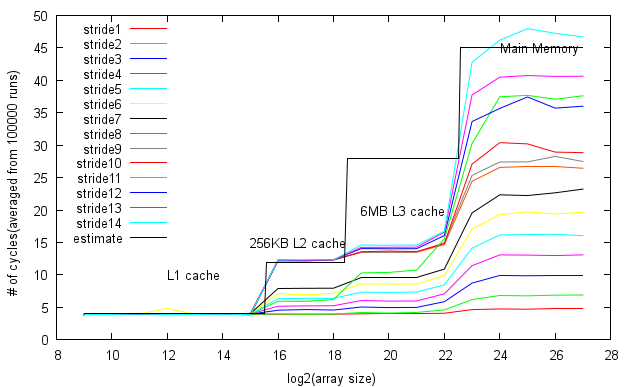
\includegraphics[scale=0.8]{memoryLatencyImage}
\end{center}
\caption {RAM latency\label{fig:access-timef}}

\end{figure}



The figure \ref{fig:access-timef} and table \ref{access-time-table} clearly indicated the average reading time for L1 cache, L2 cache, L3 cache and main memory. When the stride is small, the reading time for array of larger than L3 cache is still about the same as L1 because those data were more likely to be prefetched into the cache.

\paragraph{Success of Methodology}
We successfully replicated the result of the lmbench paper, and provided more information such as L3 cache reading time. The reason that our prediction time is actually larger than the measured time is probably because of the fact that some pre-fetching is going on when we set up the reading operation for the program. Overall, this measurement is really successful.

\subsubsection{RAM bandwidth}
\paragraph{Methodology}
We allocated an array of 128MB so that it doesn't fit into any cache (the L3 cache is 6MB).
To make the measurement, we walked through the array by incrementing a pointer to avoid summing an index and a base pointer on each iteration.
The array is filled once before the tests to ensure that the underlying pages are really allocated and to avoid TLB misses.


For the read bandwidth an integer value was read and added to an integer stored in a register.
The resulting value is printed after the measurement to avoid a compiler optimization.
For the write bandwidth, we filled the array of an arbitrary integer value.

The optimizations are turned on to reduce the number of operations not related to the memory read.
The only other operation are an incrementation of the pointer, a comparaison and a conditional jump.
All these operations are made on values stored in registers.
The compiler options -funroll-loops also helps avoid the overhead of the loop.

The measurement unit is in cycle for 128MB and is then translated to MB/s by calculating it with the CPU clock rate.
The result is averaged on 10000 iterations.

\paragraph{Predictions}
According to the specification of the RAM, the peak transfer rate is 10666 MB/s.
We are awaiting result wich should be near this value but doesn't reach this value as this is a theoritical value.
We also have a small overhead in our measurement due to the loop operations. We also expect that the writing takes about 20% higher amount of time than reading.

\paragraph{Results}
\begin{table}[h]
\begin{center}
\begin{tabular}{| l | l | l | l | l |}
\hline
Operation 		& Hardware cost & Software cost & Prediction 	& Measured \\
\hline
Read 128MB 	& 40000k cycles	& 10			& 40000k cycles	& 43494072.20 cycles \\
\hline
Write 128MB 	& 50000k cycles	& 10			& 50000k cycles	& 55758044.23 cycles \\
\hline

\end{tabular}
\end{center}

\caption{RAM bandwith\label{tab:ram-bandwidth}}
\end{table}

According to the table \ref {tab:ram-bandwidth} above, we calculated the read tranfer rate is 9711 MB/s and the write transfer rate is 7575 MB/s.

\paragraph{Success of Methodology}
Comparing to the specification of the RAM, our result is really close to the ideal transfer rate. The writing time is about 20% slower than the reading time as we expected.



\subsubsection{Page fault service time}
\paragraph{Methodology}
In order to manually create a page fault situation, we used two really large array which are the same size as main memory.
Then we filled the first array to put it into main memory first and so that the pages are allocated.
Afterwards, we filled the second array so that the first array will be totally paged out to the swap space.
The page fault service time is going to be the time it takes to get the value of an element from the first array.

We averaged the result on 10 run as more would have taken too much time.

\paragraph{Predictions}
The latency to page in a page from the disks will be really high.

The request will travers many layers :
\begin{enumerate}
\item Page fault into the solaris operating system and verifications.
\item After verification the solaris operating system will make a request on
he ZFS volume used as swap partition.
\item The request on the ZFS volume will be translated to an hypercall to the
host operating system for the block on the virtual device.
\item The host operating system will verify the call and translate the request
to a location on the logical volume associated with the virtual machine.
\item The logical volume manager of the host operating system will make a
request to the raid virtual device.
\item The raid layer will arrange the I/O and access the disk.
\item The result will go all the way back.
\end{enumerate}

The disk has an average access time of 18.7 ms but the I/O operation may be
delayed.
We except the result to be at least 100 ms due to the need to schedule the
operation.

\paragraph{Results}
\begin{table}[h]
\begin{center}
\begin{tabular}{| l | l | l | l | l |}
\hline
Operation & Hardware cost & Software cost & Prediction & Measured \\
\hline
\end{tabular}
\end{center}
\caption{Page fault service time\label{tab:page-fault}}
\end{table}

As seen in table \ref{tab:page-fault} blalba
\paragraph{Success of Methodology}

